\documentclass[8pt,xcolor=table,dvipsnames]{beamer}
\usepackage{pgfpages}
\usepackage{yhmath}
\newcommand{\Mod}[1]{\ (\mathrm{mod}\ #1)}
\providecommand{\half}{\frac{1}{2}}
\newcommand{\dg}{^\circ}
\newcommand{\arc}[1]{\wideparen{#1}}
\usetheme{Madrid}

\title{Carnot and Butterfly Theorems}
\subtitle{UMC K1, 2024}
\author{Nghia Doan}
\institute{MCC Club \& Competitions}
\date{\today}

\begin{document}

\section{Perpendicularity Lemma}

\begin{frame}[t]
    \frametitle{Carnot and Butterfly Theorems}
    \framesubtitle{Perpendicularity Lemma}
    \begin{theorem}[Perpendicularity Lemma]
        Let $AB$ and $CD$ be two intersecting lines. Then, $AB \perp CD \Longleftrightarrow CA^2 - CB^2 = DA^2 - DB^2.$
    \end{theorem}
    
    \begin{center}
        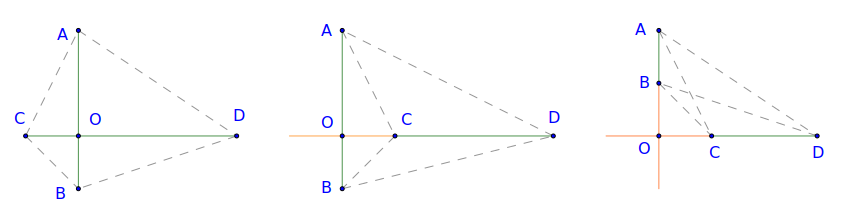
\includegraphics[width=12cm]{./svg/pdf/perpendicular-lemma.pdf}
    \end{center}

    \onslide<2->{Let $AB \perp CD.$ Let $AB \cap CD = O.$}

    \onslide<3->{$\triangle ACO,$ $\triangle BCO,$ $\triangle ADO,$ and $\triangle BDO$ are right triangles,
    by the Pythagorean Theorem:
    \[
        CA^2 - CB^2 = (OC^2 +OA^2) - (OC^2 + OB^2) = (OD^2 +OA^2) - (OD^2 + OB^2) = DA^2 - DB^2.
    \]}
\end{frame}

\begin{frame}[t]
    \frametitle{Carnot and Butterfly Theorems}
    \framesubtitle{Perpendicularity Lemma}
    \begin{center}
        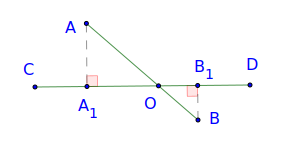
\includegraphics[width=4.5cm]{./svg/pdf/perpendicular-lemma-2.pdf}
    \end{center}

    \onslide<2->{Let $CA^2 - CB^2 = DA^2 - DB^2.$ We discuss the case where $O \in AB$ and $O \in CD.$
    Let $AA_1 \perp CD,$ and $BB_1 \perp CD.$}
    \onslide<3->{$\triangle CAA_1,$ $\triangle CBB_1,$ $\triangle DAA_1,$ and $\triangle DBB_1$ are right,
    by the Pythagorean Theorem:
    \[
        \begin{aligned}
            &CA^2 - CB^2 = DA^2 - DB^2 \Leftrightarrow (CA_1^2 + AA_1^2) - (CB_1^2 + BB_1^2) = (DA_1^2 + AA_1^2) - (DB_1^2 + BB_1^2)\\
            &\Rightarrow CA_1^2 - CB_1^2 = DA_1^2 - DB_1^2 
            \Rightarrow CA_1^2 - DA_1^2 = CB_1^2 - DB_1^2 \Rightarrow CA_1 - DA_1 = CB_1 - DB_1\\
            &\Rightarrow CA_1 - CB_1 = DA_1 - DB_1 \Rightarrow -A_1B_1 = A_1B_1 \Rightarrow A_1B_1 = 0 \Rightarrow A_1 \equiv B_1.
        \end{aligned}
    \]}

    \onslide<4->{Therefore, the perpendiculars to $CD$ from $A$ and $B$ pass through a common point on $CD,$
    so they must be the same line, i.e. $AB \perp CD.$}

    \bigbreak
    \onslide<5->{In the cases where $O$ is not between $A$ and $B$ or between $C$ and $D,$ the proof follows exactly the same steps.
    There might be a different operation when dealing with the line segments (addition or subtraction)
    depending on the configuration, but the result will always be the same.}
\end{frame}

\section{Perpendicularity Lemma - Example 1}

\begin{frame}[t]
    \frametitle{Carnot and Butterfly Theorems}
    \framesubtitle{Perpendicularity Lemma - Example 1}
    \begin{example}
        Prove that the medians $AA', BB'$ of $\triangle ABC$ are perpendicular if and only if $a^2 + b^2 = 5c^2,$
        where $AB=c, BC=a,$ and $CA=b.$
    \end{example}
    \begin{overprint}
        \onslide<1>\centering\includegraphics[width=6cm]{./svg/pdf/24-25-s9-g3-p9.pdf}
        \onslide<2->\centering\includegraphics[width=6cm]{./svg/pdf/24-25-s9-g3-p9-2.pdf}
    \end{overprint}        
    \onslide<2->{Note that $A'B'=\frac{c}{2},$ by the Perpendicularity Lemma $AA', BB'$ are perpendicular if and only if: 
    \[
        AB^2 - AB'^2 = A'B^2 - A'B'^2 \Leftrightarrow c^2 - \frac{b^2}{4} = \frac{a^2}{4} - \frac{c^2}{4} \Leftrightarrow a^2 + b^2 = 5c^2.
    \]}
\end{frame}

\section{Orthocenter of excentres is the incenter}

\begin{frame}[t]
    \frametitle{Carnot and Butterfly Theorems}
    \framesubtitle{Orthocenter of excentres is the incenter}
    \begin{example}
        Let $I_A,$ $I_B,$ and $I_C$ be the excenters opposite of $A, B,$ and $C$ in $\triangle ABC,$ respectively.
        Prove that the incenter of $\triangle ABC$ is the orthocenter of $\triangle I_A I_B I_C.$
    \end{example}
    \begin{center}
        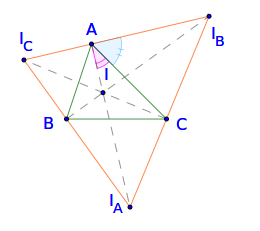
\includegraphics[width=4.5cm]{./svg/pdf/24-25-s7-g3-t4.pdf}
    \end{center}
\end{frame}

\begin{frame}[t]
    \frametitle{Carnot and Butterfly Theorems}
    \framesubtitle{Orthocenter of excentres is the incenter}
    \begin{center}
        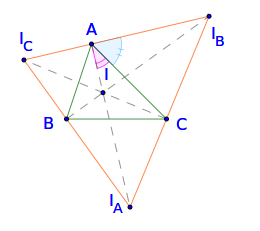
\includegraphics[width=4.5cm]{./svg/pdf/24-25-s7-g3-t4.pdf}
    \end{center}
    \onslide<2->{Let $I$ be the incenter of $\triangle ABC.$ $AI$ and $AI_B$ are internal and external angle bisectors.
    \[
        \angle IAI_B = \angle IAC + \angle CAI_B = \frac{\angle A}{2} + \frac{180\dg - \angle A}{2} = 90\dg.
    \]}

    \onslide<3->{Similarly, $\angle IAI_C = 90\dg.$ Therefore $\angle IAI_B + \angle IAI_C = 180\dg,$ thus $A \in I_B I_C,$
    and lines $I_A$ and $IA$ are the same, both are perpendicular to $I_B I_C,$ so $I_A A$ is an altitude in $\triangle I_A I_B I_C.$}

    \onslide<4->{Similar for $I_B B, I_C C$. Hence, \framebox{$I$ is the orthocenter of $\triangle I_A I_B I_C.$}}
\end{frame}

\section{Tangent Segments of the Incircle}

\begin{frame}[t]
    \frametitle{Carnot and Butterfly Theorems}
    \framesubtitle{Tangent Segments of the Incircle}
    \begin{theorem}[Tangent Segments of the Incircle]
        Let $\omega$ be the incircle in $\triangle ABC.$
        Let $D$ be the tangent point of $\omega$ to the side $BC.$ Prove that $AB+CD = AC+BD.$
    \end{theorem}
    \begin{center}
        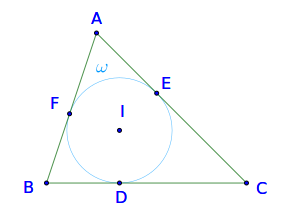
\includegraphics[width=4.5cm]{./svg/pdf/24-25-s7-g3-t3.pdf}
    \end{center}
    \onslide<2->{Let $E$ and $F$ be the tangent points of $\omega$ with the sides $CA$ and $AB,$ respectively.}
    
    \bigbreak
    \onslide<3->{$(AE, AF),$ $(BF, BD),$ and $(CD,CE)$ are pairs of tangent segments from $A, B,$ and $C$ to $\omega$, thus:
    \[
        AF = AE, BF=BD, CD = CE \Rightarrow AB+CD = AF+FB+CD = AE+EC+BD = AC + BD.
    \]}
\end{frame}

\section{Tangent Segments of the Excircles}

\begin{frame}[t]
    \frametitle{Carnot and Butterfly Theorems}
    \framesubtitle{Tangent Segments of the Excircles}
    \begin{theorem}[Tangent Segments of the Excircles]
        Let $\omega$ and $\omega_A$ be the incircle and the $A-$excircle in $\triangle ABC.$
        Let $A_1, B_1,$ and $C_1$ be the tangent points of $\omega$ with the sides $BC, CA,$ and $AB,$ respectively.
        Let $A_2, B_2,$ and $C_2$ be the tangent points of $\omega_A$ with the lines $BC, CA,$ and $AB.$ Prove that:
        \begin{enumerate}
            \item $AB + BA_2 = AC + CA_2.$
            \item $BA_2 = CA_1,$ i.e. $A_1M = MA_2,$ where $M$ is the midpoint of $BC.$
        \end{enumerate}
    \end{theorem}
    \begin{center}
        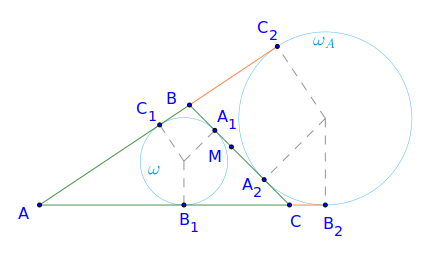
\includegraphics[width=6cm]{./svg/pdf/24-25-s7-g3-t2.pdf}
    \end{center}
\end{frame}

\begin{frame}[t]
    \frametitle{Carnot and Butterfly Theorems}
    \framesubtitle{Tangent Segments of the Excircles}
    \begin{center}
        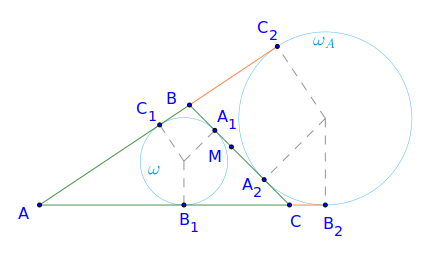
\includegraphics[width=6cm]{./svg/pdf/24-25-s7-g3-t2.pdf}
    \end{center}
    \onslide<2->{By tangent segments from $A, B,$ and $C$ to $\omega_A,$
    $AB_2 = AC_2, BA_2 = BC_2, CA_2 = CB_2.$ Thus:
    \[
        AB + AB_2 = AB + BC_2 = AC_2 = AB_2 = AC + CB_2 = AC + CA_2.
    \]}
    \onslide<3->{The sum of both sides equals the perimeter of $\triangle ABC,$
    so if $s$ denotes the semi-perimeter: \[ BA_2 = s - AB.\]}
    \onslide<4->{By the theorem Tangent Segments of the Incircle: $AC + BA_1 = AB + CA_1.$
    Similarly: \[CA_1 = s - AB \Rightarrow BA_2 = CA_1 \Rightarrow A_1M = MA_2.\]}
\end{frame}

\section{Carnot's Extended Theorem}

\begin{frame}[t]
    \frametitle{Carnot and Butterfly Theorems}
    \framesubtitle{Carnot's Extended Theorem}
    \begin{theorem}[Carnot's Extended Theorem]
        Let $P, Q,$ and $R$ be points in the plane of triangle $ABC.$
        Then, the lines $\ell_P, \ell_Q,$ and $\ell_R,$
        which are the perpendiculars from $P, Q,$ and $R$ to $BC, CA,$ and $AB,$ respectively,
        are concurrent if and only if:
        \[
            PB^2 - PC^2 + QC^2 - QA^2 + RA^2 - RB^2 = 0.
        \]
    \end{theorem}
    \begin{center}
        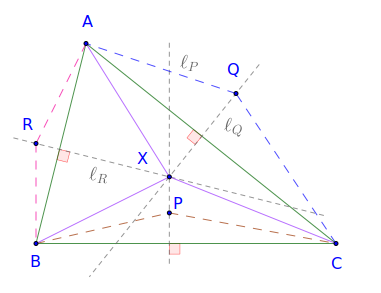
\includegraphics[width=5cm]{./svg/pdf/24-25-s7-g3-p1.pdf}
    \end{center}
\end{frame}

\begin{frame}[t]
    \frametitle{Carnot and Butterfly Theorems}
    \framesubtitle{Carnot's Extended Theorem}
    \begin{center}
        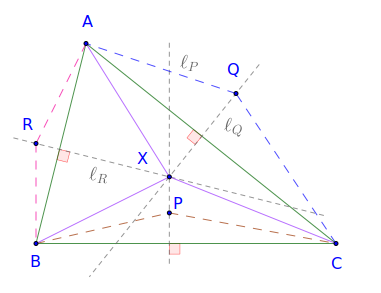
\includegraphics[width=5cm]{./svg/pdf/24-25-s7-g3-p1.pdf}
    \end{center}
    \onslide<2->{For ($\Rightarrow$), let $\ell_P, \ell_Q,$ and $\ell_R,$ be concurrent
    and let the point of concurrence be $X.$
    By the Perpendicularity Lemma, $XP \perp BC,$ so $PB^2 - PC^2 = XB^2 - XC^2,$ and similarly for others,
    then \[ XB^2 - XC^2 + XC^2 - XA^2 + XA^2 - XB^2 = 0.\]}

    \onslide<3->{Now for ($\Leftarrow$), let $PB^2 - PC^2 + QC^2 - QA^2 + RA^2 - RB^2 = 0.$ Let $X = \ell_P \cap \ell_Q.$
    Then by ($\Rightarrow$) $XB^2 - XC^2 + XC^2 - XA^2 + RA^2 - RB^2 = 0,$ or $XB^2 - XA^2 = RA^2 - RB^2,$
    so by the Perpendicularity Lemma $XR \perp AB,$ hence $\boxed{X \in \ell_R.}$}
\end{frame}

\section{Carnot's Extended Theorem - Example 1}

\begin{frame}[t]
    \frametitle{Carnot and Butterfly Theorems}
    \framesubtitle{Carnot's Extended Theorem - Example 1}
    \begin{example}
        Let $ABC$ be a triangle, and draw isosceles triangles $BCD, CAE, ABF$ externally to $ABC$,
        with $BC, CA, AB$ as their respective bases.
        Prove that the lines through $A,B,C$ perpendicular to the lines through $EF, FE,$ and $DE$, respectively, are concurrent.
    \end{example}

    \bigbreak
    \begin{center}
        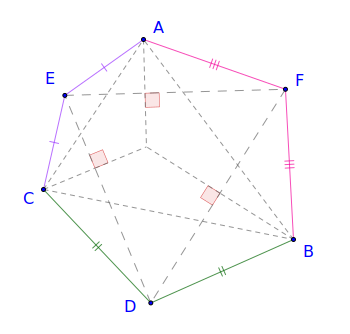
\includegraphics[width=5cm]{./svg/pdf/24-25-s7-g3-p3-0.pdf}
    \end{center}  
\end{frame}

\begin{frame}[t]
    \frametitle{Carnot and Butterfly Theorems}
    \framesubtitle{Carnot's Extended Theorem - Example 1 - Solution}
    \begin{center}
        \begin{overprint}
            \onslide<1>\centering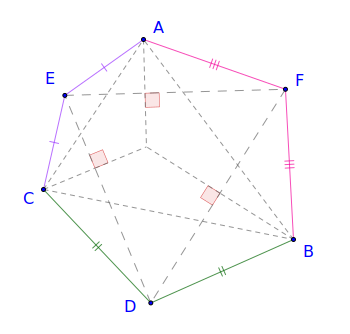
\includegraphics[width=5cm]{./svg/pdf/24-25-s7-g3-p3-0.pdf}
            \onslide<2>\centering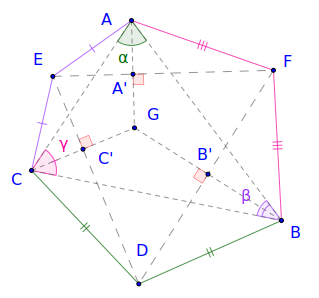
\includegraphics[width=5cm]{./svg/pdf/24-25-s7-g3-p3.pdf}
        \end{overprint}        
    \end{center}  
    \onslide<2->{Since $AE = EC, CD = DB,$ and $FB=FA,$ therefore \[ AE^2 - AF^2 + BF^2 - BD^2 + CD^2 - CE^2 = 0. \]}
    \onslide<3->{Thus by the Carnot's Extended Theorem, the lines through $A,B,C$
    perpendicular to the lines through $EF, FE,$ and $DE$, respectively, are concurrent.}
\end{frame}

\section{Carnot's Extended Theorem - Example 2}

\begin{frame}[t]
    \frametitle{Carnot and Butterfly Theorems}
    \framesubtitle{Carnot's Extended Theorem - Example 2}
    \begin{example}
        Let $I_a, I_b,$ and $I_c$ be the excenters of triangle $ABC$ opposite the vertices $A, B$ and $C,$ respectively.
        Let $A_1, B_1,$ and $C_1$ be the tangent points of the $A-, B-,$ and $C-$excircle with the sides $BC, CA,$ and $AB,$ respectively.
        Prove that the lines $I_a A_1, I_b B_1,$ and $I_c C_1$ are concurrent.    
    \end{example}

    \bigbreak
    \begin{center}
        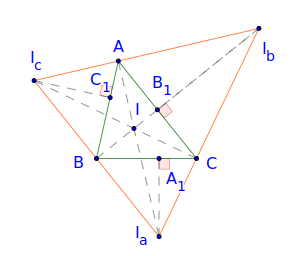
\includegraphics[width=5cm]{./svg/pdf/24-25-s7-g3-p2.pdf}
    \end{center}
\end{frame}

\begin{frame}[t]
    \frametitle{Carnot and Butterfly Theorems}
    \framesubtitle{Carnot's Extended Theorem - Example 2 - Solution}
    \begin{center}
        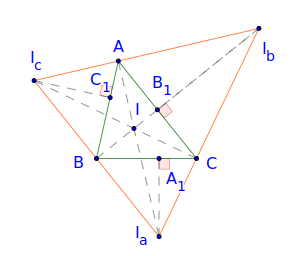
\includegraphics[width=5cm]{./svg/pdf/24-25-s7-g3-p2.pdf}
    \end{center}
    \begin{overprint}
        \onslide<2>The three perpendiculars are concurrent if and only if, by Carnot's Extended Theorem,
        \[ {I_aB}^2 - {I_aC}=^2 + {I_bC}^2 - {I_bA}^2 + {I_cA}^2 - {I_cB}^2 = 0. \]
        \onslide<3>By the theorem Tangent Segments of The Excircles, $BA_1 = s - c = AB_1,$
        where $s$ is the semi-perimeter of $\triangle ABC.$ Similarly with other sides.
        Let $x = s-c, y =s-b,$ and $z = s-a.$

        Let $r_a, r_b,$ and $r_c$ be the radii of the $A-, B-,$ and $C-$excircle, respectively.
        Then \[
            \begin{aligned}
                &{I_aB}^2 = r_a^2 + x^2,\ {I_aC}^2 = r_a^2 + y^2\\
                &{I_bC}^2 = r_b^2 + z^2,\ {I_bA}^2 = r_b^2 + x^2\\
                &{I_cA}^2 = r_c^2 + y^2,\ {I_cB}^2 = r_c^2 + z^2
            \end{aligned}
        \]
        \onslide<4>By applying Pythagorean Theorem six times:
        \[
            \underbrace{(r_a^2 + x^2)}_{{I_aB}^2} - \underbrace{(r_a^2 + y^2)}_{{I_aC}^2} + \underbrace{(r_b^2 + z^2)}_{{I_bC}^2} 
            - \underbrace{(r_b^2 + x^2)}_{{I_bA}^2} + \underbrace{(r_c^2 + y^2)}_{{I_cA}^2} - \underbrace{(r_c^2 + z^2)}_{{I_cB}^2} = 0.
        \]
        Hence, \framebox{$I_a A_1, I_b B_1,$ and $I_c C_1$ are concurrent.}
    \end{overprint}
\end{frame}

\section{Carnot's Extended Theorem - Example 3}

\begin{frame}[t]
    \frametitle{Carnot and Butterfly Theorems}
    \framesubtitle{Carnot's Extended Theorem - Example 3}
    \begin{example}
        Let $P, Q,$ and $R$ be points in the plane of triangle $ABC.$
        Then, the perpendiculars from $P, Q,$ and $R$ to $BC, CA,$ $AB,$ respectively, are concurrent if and only if
        the perpendiculars from $C, A,$ and $B$ to $PQ, QR,$ and $RP,$ respectively, are concurrent.
    \end{example}

    \bigbreak
    \begin{center}
        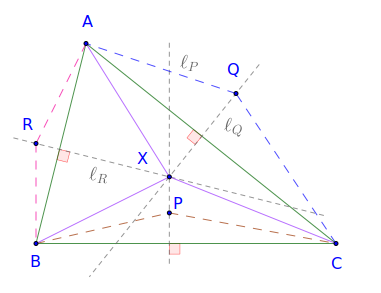
\includegraphics[width=5cm]{./svg/pdf/24-25-s7-g3-p1.pdf}
    \end{center}
\end{frame}

\begin{frame}[t]
    \frametitle{Carnot and Butterfly Theorems}
    \framesubtitle{Carnot's Extended Theorem - Example 3 - Solution}
    \begin{center}
        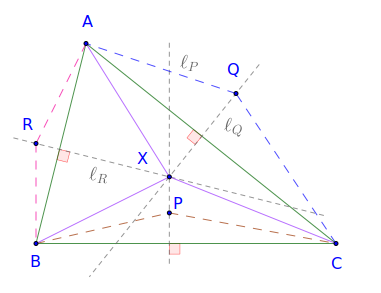
\includegraphics[width=5cm]{./svg/pdf/24-25-s7-g3-p1.pdf}
    \end{center}
    
    \onslide<2->{Let $\ell_P, \ell_Q,$ and $\ell_R,$ be the perpendiculars from $P, Q,$ and $R$ to $BC, CA,$ and $AB,$ respectively.
    By the Carnot's Extended Theorem, they are concurrent if and only if \[ PB^2 - PC^2 + QC^2 - QA^2 + RA^2 - RB^2 = 0. \]}

    \onslide<3->{Now by rearranging the terms, we have $CP^2 - CQ^2 + AQ^2 - AR^2 + BR^2 - BP^2 = 0,$
    which stands if and only if the perpendiculars from $C, A,$ and $B$ to $PQ, QR,$ and $RP,$ respectively, are concurrent.}
\end{frame}

\section{Carnot's Extended Theorem - Example 4}

\begin{frame}[t]
    \frametitle{Carnot and Butterfly Theorems}
    \framesubtitle{Carnot's Extended Theorem - Example 4}
    \begin{example}
        $ABCDEF$ is a convex hexagon such that $AB=BC, CD=DE$ and $EF=FA.$
        Prove that the angle bisectors of $\angle ABC, \angle CDE,$ and $\angle EFA$ are concurrent.
    \end{example}
    \begin{center}
        \includegraphics[width=4.3cm]{./svg/pdf/24-25-s7-g3-p5.pdf}
    \end{center}
    \onslide<2->{In $\triangle ABC,$ $AB=BC,$ thus the angle bisector of $\angle ABC$ is also the perpendicular bisector of $AC.$}
    \onslide<3->{Therefore the angle bisectors of $\angle ABC, \angle CDE,$ and $\angle EFA$ are the perpendicular bisectors of $AC, CE,$ and $EA.$}
    \onslide<4->{\framebox{They meet at $O,$ the circumcenter of $\triangle ACE.$}}
\end{frame}

\section{Carnot's Extended Theorem - Example 5}

\begin{frame}[t]
    \frametitle{Carnot and Butterfly Theorems}
    \framesubtitle{Carnot's Extended Theorem - Example 5}
    \begin{example}
        Three circles intersect pairwise as shown.
        Prove that $AD$, $BE$, and $CF$ are concurrent.
    \end{example}
    \begin{center}
        \begin{overprint}
            \onslide<1>\centering\includegraphics[width=8cm]{./svg/pdf/24-25-t2-p14.pdf}
            \onslide<2>\centering\includegraphics[width=8cm]{./svg/pdf/24-25-t2-p14-2.pdf}
        \end{overprint}        
    \end{center}
    \onslide<2->{Since $O_1 O_2 \perp AD,$ $O_2O_3 \perp BE,$ $O_3O_1 \perp CF,$
    and $AO_1^2 - AO_2^2 + BO_2^2 - BO_3^2 + CO_3^2 - CO_1^2 = 0.$
    By the Carnot's Extended Theorem, $AD$, $BE$, and $CF$ are concurrent.}
\end{frame}

\section{The Butterfly Theorem}

\begin{frame}[t]
    \frametitle{Carnot and Butterfly Theorems}
    \framesubtitle{The Butterfly Theorem}
    \begin{theorem}[Butterfly Theorem]
        \label{problem:24-25-S2-G3-P1}
        Let $M$ be the midpoint of a chord $PQ$ of a circle $\omega,$ through which two other chords $AB$ and $CD$ are drawn.
        Let $AD \cap PQ = X$ and $BC \cap PQ = Y.$ Prove that $M$ is also the midpoint of $XY.$
    \end{theorem}
    
    \begin{center}
        \includegraphics[width=3cm]{./png/24-25-s2-g3-p1.png}
    \end{center}

    \onslide<2->{Let $\omega$'s center $O.$ $MP=MQ,$ so $OM \perp PQ.$ 
    To prove $XM = MY,$ we need $\angle MOX = \angle MOY.$}
    \onslide<3->{Let $OR \perp AD$ and $OS \perp BC$, then $AR = RD$ and $BS = SC.$}
    \onslide<4->{\[
        \begin{aligned}
            &\angle DAM \equiv \angle DAB \stackrel{\omega}{=} \angle DCB \equiv \angle MCB\ \text{and}\ \angle AMD = \angle CMB\\
            &\Rightarrow \triangle AMD \sim \triangle CMB \Rightarrow \frac{AD}{AM} = \frac{CB}{CM}\\
        \end{aligned}
    \]}
\end{frame}

\begin{frame}[t]
    \frametitle{Carnot and Butterfly Theorems}
    \framesubtitle{The Butterfly Theorem}
    \begin{center}
        \includegraphics[width=3cm]{./png/24-25-s2-g3-p1.png}
    \end{center}
    \[
        \begin{aligned}
            &\frac{AD}{AM} = \frac{CB}{CM} \Rightarrow \frac{2AR}{AM} = \frac{2CS}{CM} \Rightarrow \frac{AR}{AM} = \frac{CS}{CM} \Longrightarrow \triangle AMR \sim \triangle CMS
            \Rightarrow \angle MRA = \angle MSC \quad (*)
        \end{aligned}
    \]
    
    \bigbreak
    \onslide<2->{Since $OM \perp PQ,$ $OR \perp AD,$ and $\angle ORX + \angle OMX = 180^{\circ},$
    so $OMXR$ is a cyclic quadrilateral. Similarly $OMYS$ is also a cyclic quadrilateral.}

    \bigbreak
    \onslide<3->{Therefore,
    \[
        \angle MOX \stackrel{OMXR}{=} \angle MRX \equiv \angle MRA \stackrel{(*)}{=} \angle MSC \equiv \angle MSY  \stackrel{OMYS}{=} \angle MOY.
    \]}

    \onslide<4->{Thus $\triangle MXO \cong \triangle MYO,$ or $MX = MY,$ thus \framebox{$M$ is also the midpoint of $XY.$}}
\end{frame}

\section{The Butterfly Theorem in converse}

\begin{frame}[t]
    \frametitle{The Butterfly Theorem}
    \framesubtitle{The Butterfly Theorem in converse}
    \begin{theorem}[The Butterfly Theorem in converse]
        Denote by $M$ the point of intersection of the chords $AB$ and $CD$ of a circle $\omega.$
        
        \bigbreak
        $\ell$ is a line passing through $M$ such that $X = AD\cap \ell$ and $Y = BC \cap \ell,$ and $MX = MY.$
        
        \bigbreak
        Then $OM \perp \ell.$
    \end{theorem}
    
    \begin{center}
        \includegraphics[width=3cm]{./png/24-25-s2-g3-p1.png}
    \end{center}
\end{frame}

\section{The Butterfly Theorem - Example 1}

\begin{frame}[t]
    \frametitle{Carnot and Butterfly Theorems}
    \framesubtitle{The Butterfly Theorem - Example 1}
    \begin{example}
        $(O)$ and $(I)$ are circumcircle and incircle, respectively, of $\triangle ABC.$
        Lines through $BI$ and $CI$ intersect $(O)$ at $E$ and $F,$respectively.
        Let $K$ and $D$ be the intersections of $AI$ with $EF$ and $BC.$
        If $AB + AC = 2BC,$ prove that $IK = ID.$
    \end{example}

    \bigbreak
    \begin{center}
        \includegraphics[width=5cm]{./svg/pdf/24-25-s2-g3-p5.pdf}
    \end{center}
\end{frame}

\begin{frame}[t]
    \frametitle{Carnot and Butterfly Theorems}
    \framesubtitle{CThe Butterfly Theorem - Example 1 - Solution}
    \begin{center}
        \includegraphics[width=5cm]{./svg/pdf/24-25-s2-g3-p5-2.pdf}
    \end{center}
    \begin{overprint}
        \onslide<2>Let $M$ be the intersection of $AI$ and the circle $(O),$ $M \equiv A.$ See above on the right.
        \[
            \angle AMC = \angle ABD, \angle BAD = \angle CAM \Rightarrow \triangle BAD \sim \triangle MAC \Rightarrow \frac{MC}{MA} = \frac{BD}{BA}.
        \]
        \onslide<3>Note that $BI$ is the angle bisector in $\triangle DBA,$ and $CI$ is the angle bisector in $\triangle DCA,$ so 
        \[
            \frac{BD}{BA} = \frac{ID}{IA} = \frac{CD}{CA} = \frac{BD + CD}{BA + CA} = \frac{BC}{2BC} = \frac{1}{2}
            \Rightarrow MA = 2MC.
        \]
        \onslide<4>Furthermore $\angle MIC = \frac{\angle A + \angle C}{2} = \angle ICM,$ thus $\triangle MIC$ is isosceles at $M,$
        so $MI = MC.$ therefore $MI = \half MA,$ so $MI = IA.$   
        
        Consider the circle $(O).$ Chords $BE$ and $CF$ intersecting at $I.$ A line through $I$ intersects $BC$ and $EF$ at $D$ and $K,$ respectively.
        Since $IM = IA,$ by the \textit{Butterfly Theorem} $\boxed{IK = ID.}$
    \end{overprint}        
\end{frame}

\section{The Butterfly Theorem - Example 2}

\begin{frame}[t]
    \frametitle{Carnot and Butterfly Theorems}
    \framesubtitle{The Butterfly Theorem - Example 2}
    \begin{example}
        The radii of the circles $\omega$ and $\gamma$ have the same length. The circles intersect each other at $A$ and $B.$
        Let $O$ be the midpoint of $AB.$ Chord $CD$ of $\omega$ through $O$ intersects $\gamma$ at $P.$
        Chord $EF$ of $\gamma$ through $O$ intersects $\omega$ at $Q.$
        Prove that $AB,$ $CQ,$ and $EP$ are concurrent.
    \end{example}

    \bigbreak
    \begin{center}
        \includegraphics[width=8cm]{./svg/pdf/24-25-s2-g3-p6.pdf}
    \end{center}
\end{frame}

\begin{frame}[t]
    \frametitle{Carnot and Butterfly Theorems}
    \framesubtitle{CThe Butterfly Theorem - Example 2 - Solution}
    \begin{center}
        \includegraphics[width=8cm]{./svg/pdf/24-25-s2-g3-p6-2.pdf}
    \end{center}
    \begin{overprint}
        \onslide<2>Let $H$ and $K$ be the second intersections of $CD$ and $EF$ with $\gamma$ and $omega,$ respectively.
        Let $S = CQ \cap AB,$ $S' = EF \cap AB,$ and $M = DK \cap AB.$
        \onslide<3>Consider the circle $\omega,$ chords $CD$ and $KQ$ intersecting at $O.$ A line through $O$ intersects $CQ$ and $KD$ at $S$ and $M,$ respectively.
        Since $OA = OA,$ by the \textit{Butterfly Theorem} $OS = OM.$ 
        \onslide<4>Now, the radii of the circles $\omega$ and $\gamma$ have the same length,
        thus $O$ is midpoint of $PD$ ($\triangle IOP \cong \triangle I'OD$) and $KE.$
        Therefore $PKDE$ is a parallelogram, so $OS' = OM.$
        
        Hence, $AB,$ $CQ,$ and $EP$ are concurrent.
    \end{overprint}        
\end{frame}

\end{document}
